\documentclass[journal,12pt,onecolumn]{IEEEtran}
\usepackage{cite}
\usepackage{amsmath,amssymb,amsfonts,amsthm}
\usepackage{algorithmic}
\usepackage{graphicx}
\usepackage{textcomp}
\usepackage{xcolor}
\usepackage{txfonts}
\usepackage{listings}
\usepackage{enumitem}
\usepackage{mathtools}
\usepackage{gensymb}
\usepackage{comment}
\usepackage[breaklinks=true]{hyperref}
\usepackage{tkz-euclide} 
\usepackage{listings}
\usepackage{gvv}      
\usepackage[latin1]{inputenc}                                
\usepackage{color}                                            
\usepackage{array}                                            
\usepackage{longtable}                                       
\usepackage{calc}                                             
\usepackage{multirow}    
\usepackage{hhline}                                           
\usepackage{ifthen}     
\usepackage{lscape}
\usepackage{tabularx}
\usepackage{array}
\usepackage{float}
\usepackage{multicol}
\usepackage{tikz}
\usepackage{pgfplots}
\pgfplotsset{compat=1.18} % or

\newtheorem{theorem}{Theorem}[section]
\newtheorem{problem}{Problem}
\newtheorem{proposition}{Proposition}[section]
\newtheorem{lemma}{Lemma}[section]
\newtheorem{corollary}[theorem]{Corollary}
\newtheorem{example}{Example}[section]
\newtheorem{definition}[problem]{Definition}
\newcommand{\BEQA}{\begin{eqnarray}}
\newcommand{\EEQA}{\end{eqnarray}}
\newcommand{\define}{\stackrel{\triangle}{=}}
\theoremstyle{remark}
\newtheorem{rem}{Remark}

\begin{document}
\bibliographystyle{IEEEtran}

\title{CE : GATE 2014}
\author{ai24btech11014 \\ Charitha Sri}
\maketitle

\section{SET-1}

\begin{enumerate}
    \item An isolated three-phase traffic signal is designed by Webster's method. The critical flow ratio for three phases are $0.20, 0.30,$ and $0.25$ respectively, and lost time per phase is 4 seconds. The optimum cycle length (in seconds) is \underline{\hspace{1cm}}.
 
    \item A levelling is carried out to establish the Reduced Levels (RL) of point R with respect to the Bench Mark (BM) at P. The staff readings taken are given below. \\
 \begin{table}[h]
        \centering
        \begin{tabular}{ c@{\hskip 1cm }c }
            Group I & Group II \\
            P. Alidade & 1. Chain surveying \\
            Q. Arrow & 2. Levelling \\
            R. Bubble tube & 3. Plain table surveying \\
            S. Stadia hair & 4. Theodolite surveying \\
        \end{tabular}
    \end{table}


    If RL of P is +100.000m, then RL (in m) of R is:
    \begin{enumerate}
        \begin{multicols}{2}
            \item $103.355$
            \item $103.155$
            \item $101.455$
            \item $100.355$
        \end{multicols}
    \end{enumerate}

    \item Group I lists tools/instruments, while Group II lists the corresponding surveying methods. Match the tool/instrument with the corresponding method of surveying.
   \begin{table}[h]
        \centering
        \begin{tabular}{ c@{\hskip 1cm }c }
            Group I & Group II \\
            P. Alidade & 1. Chain surveying \\
            Q. Arrow & 2. Levelling \\
            R. Bubble tube & 3. Plain table surveying \\
            S. Stadia hair & 4. Theodolite surveying \\
        \end{tabular}
    \end{table}


    \begin{enumerate}
        \begin{multicols}{2}
            \item P-3; Q-2; R-1; S-4
            \item P-2; Q-4; R-3; S-1
            \item P-1; Q-2; R-4; S-3
            \item P-3; Q-1; R-2; S-4
        \end{multicols}
    \end{enumerate}

\end{enumerate}
\section{SET-2}
\begin{enumerate}
    \item A fair (unbiased) coin was tossed four times in succession and resulted in the following outcomes: (i) Head, (ii) Head, (iii) Head, (iv) Head. The probability of obtaining a 'Tail' when the coin is tossed again is:
    \begin{enumerate}
        \begin{multicols}{4}
            \item $0$
            \item $\frac{1}{2}$
            \item $\frac{4}{5}$
            \item $\frac{1}{5}$
        \end{multicols}
    \end{enumerate}


\item The determinant of the matrix $\begin{pmatrix}
0 && 1 && 2 && 3 \\ 1 && 0 && 3 && 0 \\ 2 && 3 && 0 && 1 \\ 3 && 0 && 1 && 2 \end{pmatrix}$ is \underline{\hspace{1cm}}

\item $ z = \frac{2 - 3 i}{-5 + i}$ can be expressed as
\begin{enumerate}
    \begin{multicols}{2}
    \item $ -0.5 - 0.5i $
     \item $-0.5 + 0.5i$
      \item $0.5 - 0.5i$
       \item $0.5 + 0.5i$
    \end{multicols}
\end{enumerate}

\item The integrating factor for the differential equation $\frac{dP}{dt} + k_{2}P = k_{1}L_{0} e^{-k_{1}t}$ is 
\begin{enumerate}
\begin{multicols}{4}
    \item $e^{-k_{1}t}$
    \item $e^{-k_{2}t}$
     \item $e^{k_{1}t}$
    \item $e^{k_{2}t}$
\end{multicols}
\end{enumerate}

\item If $\brak{x}$ is a continuous, real valued random variable defined over the interval $\brak{-\infty, + \infty}$ and its occurence is defined by the density function given as: $f\brak{x} = \frac{1}{\sqrt{2 \pi}}b e^{\frac{-1}{2} {\brak{\frac{x - a}{b}}}^{2}}$ where $'a'$ and $'b'$ are the statistical attributes of the random variable $\brak{x}$. The value of the integral $\int_{-\infty}^{a} \frac{1}{\sqrt{2 \pi}}b e^{\frac{-1}{2} {\brak{\frac{x - a}{b}}}^{2}} dx$ is 

\begin{enumerate}
\begin{multicols}{4}
 \item $1$
 \item $0.5$
 \item $\pi$
 \item $\frac{\pi}{2}$
\end{multicols}
\end{enumerate}

\item Group I contains representative stress-strain curves as shown in the figure, while Group II gives the list of materials. Match the stress-strain  curves with the corresponding materials.

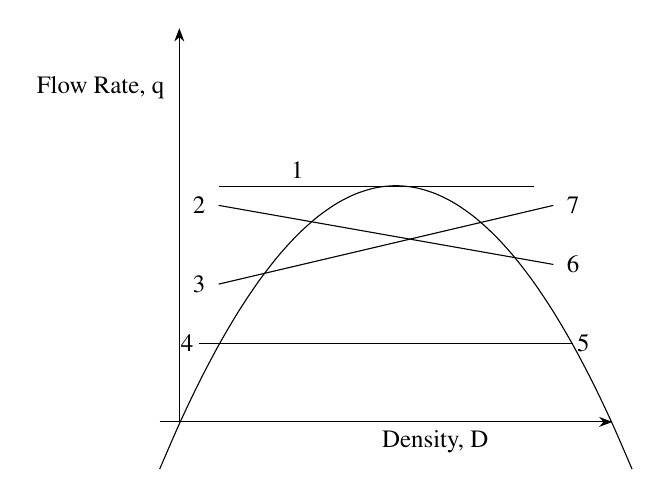
\begin{tikzpicture}

% Arrows for flow
\draw [->, >=Stealth] (6,9.5) -- (11.75,9.5);
\draw [->, >=Stealth] (6.25,9.5) -- (6.25,14.5);

% Labels for density and flow rate
\node [font=\small] at (9.5,9.25) {Density, D};
\node [font=\small] at (5.25,13.75) {Flow Rate, q};

% Short lines representing segments
\draw [-] (6.75,12.49) -- (10.75,12.49);
\draw [-] (6.75,11.25) -- (11,12.25);
\draw [-] (6.75,12.25) -- (11,11.5);
\draw [-] (6.5,10.5) -- (11.25,10.5);

% Labels for points
\node [font=\small] at (7.75,12.7) {1};
\node [font=\small] at (6.5,12.25) {2};
\node [font=\small] at (11.25,12.25) {7};
\node [font=\small] at (6.5,11.25) {3};
\node [font=\small] at (11.25,11.5) {6};
\node [font=\small] at (11.38,10.5) {5};
\node [font=\small] at (6.35,10.5) {4};

% Downward-opening parabola that passes through (6.5, 9.5) and (11.5, 9.5)
\draw[domain=6:12,smooth,variable=\x,black] plot (\x,{-(0.4*(\x - 9)^2) + 12.5}); 


\end{tikzpicture}

\begin{table}[h]
        \centering
        \begin{tabular}{ c@{\hskip 1cm }c }
            Group I & Group II \\
            P. Alidade & 1. Chain surveying \\
            Q. Arrow & 2. Levelling \\
            R. Bubble tube & 3. Plain table surveying \\
            S. Stadia hair & 4. Theodolite surveying \\
        \end{tabular}
    \end{table}


    \begin{enumerate}
        \begin{multicols}{2}
            \item P-1; Q-3; R-2; 
            \item P-2; Q-3; R-1; 
            \item P-3; Q-1; R-2; 
            \item P-3; Q-2; R-1; 
        \end{multicols}
    \end{enumerate}

\item The first moment of area about the axis of bending for a beam cross-section is
   \begin{enumerate}
        \begin{multicols}{2}
        \item moment of inertia
        \item section modulus
        \item shape factor
        \item polar moment of inertia 
        \end{multicols}
    \end{enumerate}

    \item Polar moment of inertia $\brak{I_{P}}$ , in $cm^{4}$, of a rectangular section having width, $ b = 2 cm $ and depth $ d = 6 cm $  is \underline{\hspace{2cm}} 
    \item The target mean strength $f_{cm}$ for concrete mix design obtained from the charecteristic strength $f_{ck}$  and standard deviation $\sigma$, as defined in IS:456-2000, is
    \begin{enumerate}
        \begin{multicols}{2}
            \item $f_{ck} + 1.35 \sigma $
            \item $f_{ck} + 1.45 \sigma $
            \item $f_{ck} + 1.55 \sigma $
            \item $f_{ck} + 1.65 \sigma $
        \end{multicols}
    \end{enumerate}

\item The flexural tensile strength of M25 grade of concrete, in $N/mm^{2}$ as per IS:456-2000 is \underline{\hspace {1 cm}}


\end{enumerate}
\end{document}
